% Beamer Presentation and Lecture Note Template
% Version 0.1
% by Paul Vesey

\mode<presentation> {
\usetheme{Antibes}
\setbeamercovered{invisible}
\setbeamertemplate{footline}[frame number]
\setbeamertemplate{navigation symbols}{} 
}

\usepackage{eurosym}
\usepackage{graphicx}
\usepackage{wasysym}
\usepackage{hyperref}
\usepackage{amsmath}
\usepackage{amssymb}
\usepackage{mathtools}
\usepackage{tikz}
\usepackage{pgf}
\usepackage{pgfplots}
\usepackage{pxfonts}
\usepackage{textcomp}
\usepackage{verbatim}
\usepackage{color}
\usepackage{xcolor}
\usepackage{fix-cm}


\author{Paul Vesey}
\institute[TUS]
{
Technological University of the Shannon \\
\medskip
{\emph{paul.vesey@tus.ie}}
}
\date{Autumn 2022}




\title[Project Management]{Project Quality Management}


\begin{document}
%
\usetikzlibrary{arrows}
\usepgflibrary{patterns}

\tableofcontents
\newpage



\begin{frame}
\titlepage
\end{frame}\begin{center}\line(1,0){250}\end{center}
%
%








\section{Project Quality Management}

\subsection{Introduction}

\begin{frame}
\frametitle{Project Quality Management}
Project Quality Management Processes include all activities of the performing organisation that determine quality policy, objectives, and responsibilities so that the project will satisfy the needs for which it was undertaken.\\
Processes are:\\
\begin{itemize}
	\item Plan Quality
	\item Perform Quality Assurance
	\item Perform Quality Control
\end{itemize}
\end{frame}




\begin{frame}
\frametitle{Project Quality Management}
PMBOK processes are intended to be compatible with International Organisation for Standardisation (ISO) standards.\\
Other Standards include:\\
\begin{itemize}
	\item Total Quality Management (TQM)
	\item Six Sigma
	\item Failure Mode \& Effect Analysis
	\item Etc.
\end{itemize}
\end{frame}




\begin{frame}
\frametitle{Project Quality Management}
\begin{itemize}
	\item Project Quality Management must address the management of projects and the product of the project.
	\item Project Quality Management applies to all projects regardless of the nature of the product.
	\item Project Quality Techniques are specific to the particular type of product produced by the project.
\end{itemize}
\end{frame}




\begin{frame}
\frametitle{Project Quality Management}

Quality is:
\begin{itemize}
\item �the degree to which a set of inherent characteristics fulfill requirements�, American Society for Quality, 2000
\end{itemize}
The critical element is to turn stakeholder needs, wants and expectations into requirements through Stakeholder Analysis, performed during Project Scope Management
\end{frame}




\begin{frame}
\frametitle{Quality and Grade}
\textbf{Quality} and \textbf{Grade} are not the same.  \\
Grade is a category assigned to products or services having the same functional use but different technical characteristics. \\
\hspace{1cm} 5$\star$ Hotel\\
\hspace{1cm} 2$\star$ Hotel\\
Both serve the same function (provide a bed) but differ greatly technically.
\begin{itemize}
	\item Low Quality is always a problem
	\item Low Grade may not be a problem
\end{itemize}
Ryan Air: low grade (no frills), high quality.
\end{frame}




\begin{frame}
\frametitle{Precision and Accuracy}
\textbf{Precision} and \textbf{Accuracy} are not the same.\\
Precision is consistency that the value of repeated measurements are clustered and have little scatter
\begin{itemize}
	\item Multiple Unit similarity
\end{itemize}
Accuracy is how `close' the measured value is to the real value
\begin{itemize}
	\item Measurement Error
\end{itemize}
Inaccurate measurement can yield false precision
\end{frame}




\begin{frame}
\frametitle{QM and PM}
Quality Management and Project Management both recognize the importance of:
\begin{itemize}
	\item Customer Satisfaction
	\item Prevention over Inspection
	\item Management Responsibility
	\item Continuous Improvement
\end{itemize}
\end{frame}


\subsection{Plan Quality}

\begin{frame}
\frametitle{Plan Quality}{Part of the Planning Process Group}
\begin{figure}
	\centering
		\includegraphics[width = 10cm]{images/fig8-3.jpg}
	\label{fig:8-3}
\end{figure}

\end{frame}




\begin{frame}
\frametitle{Plan Quality}
\textit{`Quality is Planned, Designed, and Built in - Not Inspected in.'}\\
Quality Planning involves identifying which quality standards are relevant to the project and determining how to satisfy them.\\
Quality Planning should be performed in parallel with all other planning processes\\
\begin{itemize}
	\item If high grade finished are required, then high grade resources (employees and/or subcontractors) need to be used in order to achieve the quality objective of `high grade finish'
\end{itemize}
\end{frame}




\begin{frame}
\frametitle{Plan Quality \hfill Inputs}
Enterprise Environmental Factors\\
\begin{itemize}
	\item Government Rules, Standards, Regulations,
	\item Industry Best Practice etc.
\end{itemize}
Organisational Process Assets\\
\begin{itemize}
	\item Performing Organisations Quality Policies, Procedures, Guidelines etc.
	\item If they do not exist, the PM team needs to generate them
\end{itemize}
\end{frame}




\begin{frame}
\frametitle{Plan Quality \hfill Inputs}
Scope Baseline\\
\begin{itemize}
	\item Details Major Deliverables, Project Objectives, Thresholds, and Acceptance Criteria
	\item Thresholds: limits of cost, time, resources
	\item Acceptance Criteria: performance requirements and essential conditions that must be met before project deliverables are accepted
	\item Etc.
\end{itemize}
Refer to Book
\end{frame}




\begin{frame}
\frametitle{Plan Quality \hfill Tools and Techniques}
\textbf{Cost - Benefit Analysis (CBA)}\\
\begin{itemize}
	\item Remember Ford Pinto?  Cost of improved quality must be less than the potential savings or benefit
	\item Benefits can be realised by less Rework, Higher Productivity, increased stakeholder satisfaction (clients and employees)
\end{itemize}
	
\textbf{Benchmarking }

\begin{itemize}
	\item Comparing actual or planned projects practices to those of other projects to generate ideas for improvement and to provide a basis by which to measure performance: Dominos Pizza
\end{itemize}
\end{frame}

Domino's Pizza, and other similar organisations are a model for efficiency.  They can take an order, assemble and cook the product, and deliver it to your home within an hour.  Most organisations can only dream of this level of efficient production and logistics.  Recently, they have also been highly successful in implementing on-line order processing.  The Australian business unit is currently taking 50\% of their orders on-line, and expect this to grow to 80\% over the next 3 years.



\begin{frame}
\frametitle{Plan Quality \hfill Tools and Techniques}
\textbf{Design of Experiments (DOE)}\\
\begin{itemize}
	\item Statistical Method that helps identify which factors may influence specific variables of a product or process under development.
	\item Also used for optimisation of processes
	\item Provides a framework that can be used to modify several important factors in parallel
\end{itemize}
\textbf{Cost of Quality (COQ)}
\begin{itemize}
	\item Total Costs incurred by investment in preventing non-conformance to requirements, appraising the product or service, etc.
	\item Failure Costs are often split into Internal Costs and External Costs
\end{itemize}
\end{frame}




\begin{frame}
\frametitle{Plan Quality \hfill Tools and Techniques}
\textbf{Quality Planning Tools:}
\begin{itemize}
	\item Brainstorming
	\item Affinity Diagrams
	\item Matrix Diagrams
	\item Etc.
\end{itemize}
\textbf{Control Charts:}
\begin{itemize}
	\item See next slide and refer to book
\end{itemize}	
\end{frame}




\begin{frame}
\frametitle{Control Charts}
\begin{figure}
	\centering
		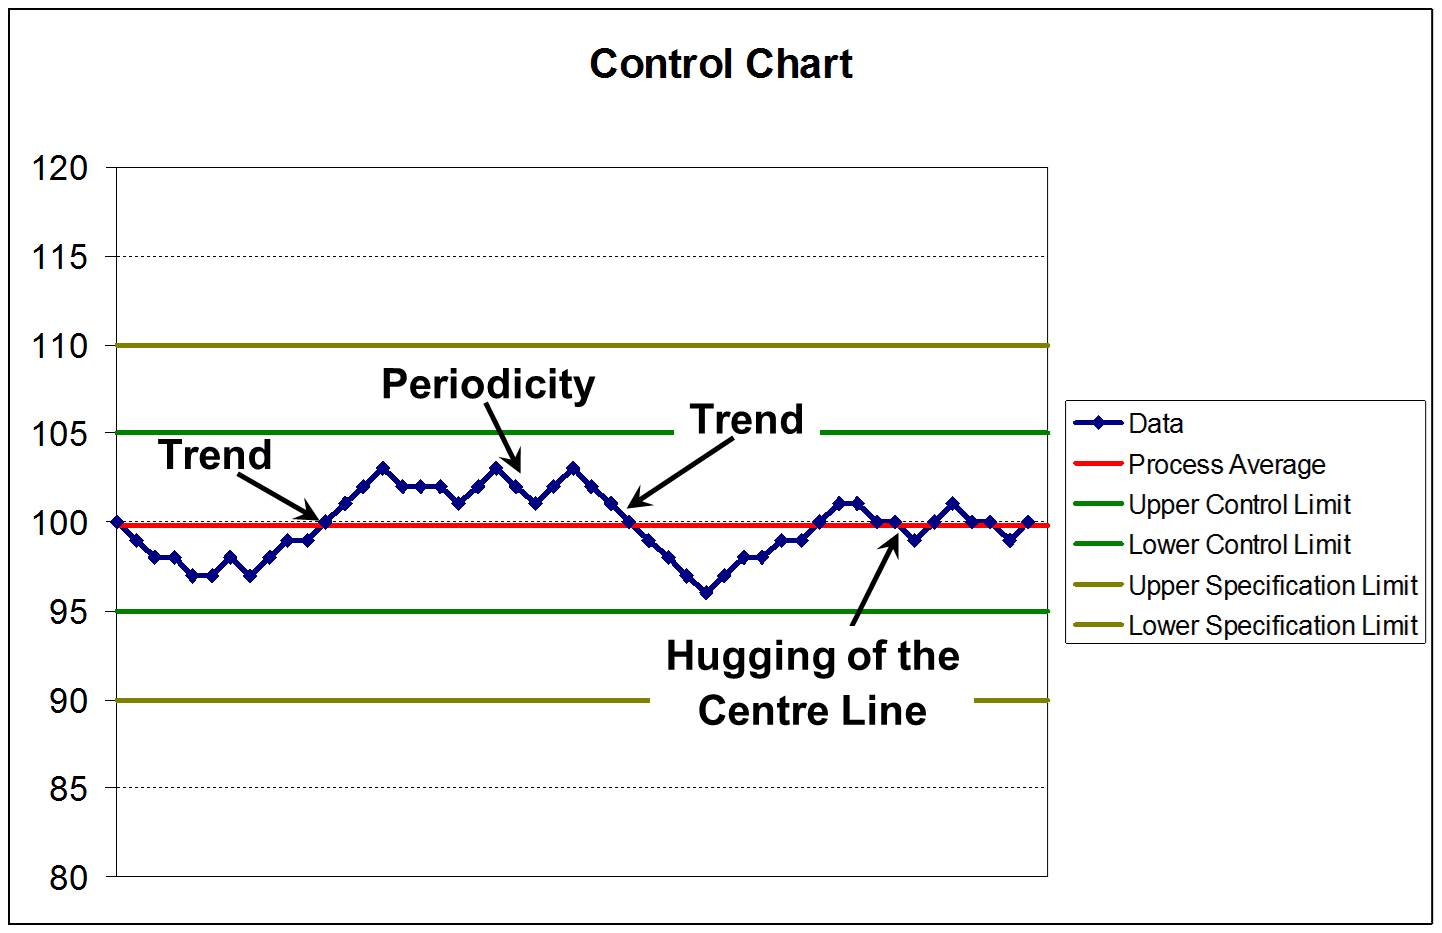
\includegraphics[width = 10cm]{images/controlchart.jpg}
	\label{fig:contolchart}
\end{figure}
\end{frame}




\begin{frame}
\frametitle{Plan Quality \hfill Outputs}

\textbf{Quality Management Plan:}
\begin{itemize}
	\item Describes how the PM team will implement the Quality Policy
	\item QM Plan is an input to the overall PM Plan
\end{itemize}
\textbf{Quality Metrics:}
\begin{itemize}
	\item An Operational Definition that describes, in very specific terms, what something is and how the quality control process measures it.
\end{itemize}	
\textbf{Quality Checklists:}
\begin{itemize}
	\item A structured tool used to verity that a set of required steps has been performed, very common in H\&S
\end{itemize}
\end{frame}




\begin{frame}
\frametitle{Plan Quality \hfill Outputs}
\textbf{Process Improvement Plan:}
\begin{itemize}
	\item Subsidiary of the PM Plan
	\item Details Steps for Analysing Processes that will facilitate the identification of waste and non-value added activity.
\end{itemize}
\textbf{Project Document Updates}
\begin{itemize}
	\item As per book
\end{itemize}
\end{frame}










\begin{frame}
\frametitle{Perform Quality Assurance}
Part of the Executing Process Group
\begin{figure}
	\centering
		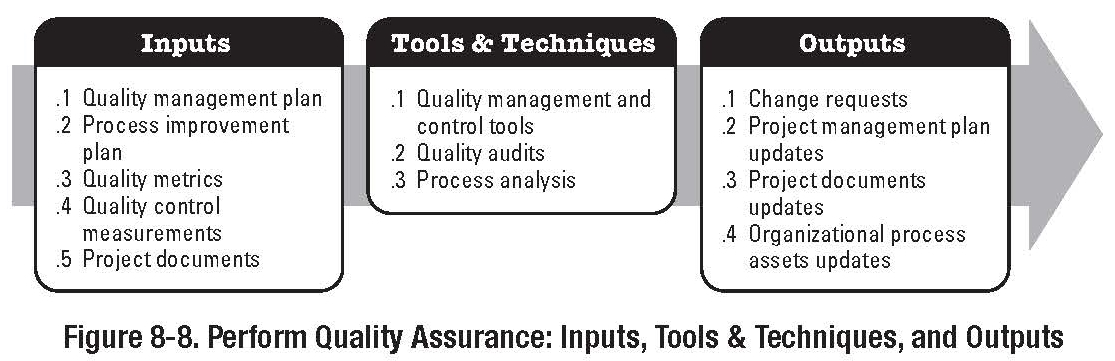
\includegraphics[width = 10cm]{images/Fig8-8.jpg}
	\label{fig:8-8}
\end{figure}
\end{frame}




\begin{frame}
\frametitle{Perform Quality Assurance}
\begin{itemize}
	\item Quality Assurance is the application of planned, systematic quality activities to ensure that the project will employ all processes needed to meet requirements.
	\item Quality Assurance is about implementing systems and procedures that will lead to fulfilment of project objectives and deliverables.
\end{itemize}
\end{frame}




\begin{frame}
\frametitle{Perform Quality Assurance \hfill Inputs}
\textbf{Project Management Plan}
\begin{itemize}
	\item Quality Plan, etc. refer to book
	\item Process Improvement Plan
\end{itemize}
\textbf{Quality Metrics}
\begin{itemize}	
	\item Already covered, refer to book
\end{itemize}
\textbf{Work Performance Information}
\begin{itemize}
	\item Work Performance Information including technical performance measures, project deliverable status, required corrective actions, performance reports, etc. EVMS yields performance information in relation to costs and schedules
\end{itemize}
\end{frame}




\begin{frame}
\frametitle{Perform Quality Assurance \hfill Inputs}
\textbf{Quality Control Measurements}
\begin{itemize}
	\item Results of the Quality Control Activities.
	\item Results are fed back into fed back into the QA process to determine the success of Corrective Actions, and to determine if changes to the QA process are successful
\end{itemize}
\end{frame}




\begin{frame}
\frametitle{Perform Quality Assurance \hfill Tools and Techniques}
The tools and techniques for quality planning can be applied to quality assurance\\
\textbf{Quality Audits:}
\begin{itemize}
	\item Structured, independent review to determine whether project activities comply with organisational and project policies, processes and procedures. for instance Reuters PCB Quality policy required that tracks on PCB's should could only change direction in two $45^\circ$ steps. 
\end{itemize}
\begin{figure}
	\centering
		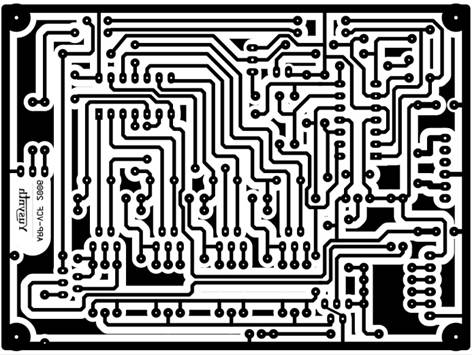
\includegraphics[width = 3cm]{images/pcb.jpg}
	\label{fig:pcb}
\end{figure}
\end{frame}




\begin{frame}
\frametitle{Perform Quality Assurance \hfill Tools and Techniques}
\textbf{Process Analysis}
\begin{itemize}
	\item Process Analysis follows the steps outlined in the process improvement plan to identify needed improvements from an organisational and technical standpoint
\end{itemize}
Most Business Processes could be improved by analysis
\begin{itemize}
	\item Purchase Order Processing; value under \euro1000.00
	\item Technical Processes can be more difficult to analyse
	\item Includes Root Cause Analysis etc.
\end{itemize}
\end{frame}




\begin{frame}
\frametitle{Perform Quality Assurance \hfill Outputs}
\begin{itemize}
	\item Organisational Process Assets Updates
	\item Change Requests
	\item Recommended Corrective Actions
\begin{itemize}	
	\item Corrective Actions is an action that is recommended immediately as a result of QA audits and processes
\end{itemize}
	\item Project Management Plan Updates
	\item Project Document Updates
\end{itemize}
\end{frame}




\begin{frame}
\frametitle{Control Quality}
Part of the Monitoring and Controlling Process Group
\begin{figure}
	\centering
		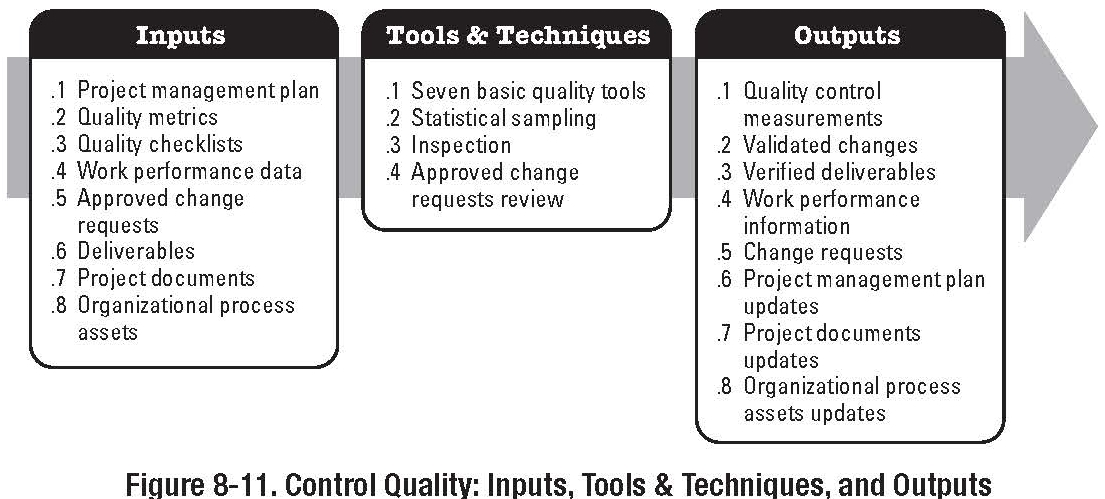
\includegraphics[width = 10cm]{images/Fig8-11.jpg}
	\label{fig:8-11}
\end{figure}
\end{frame}




\begin{frame}
\frametitle{Perform Quality Control}
\begin{itemize}
	\item Quality Control involves monitoring specific project results to determine whether they comply with relevant quality standards.
	\item Also involves identifying ways to eliminate causes of unsatisfactory results.
\end{itemize}
\end{frame}




\begin{frame}
\frametitle{Perform Quality Control}
PM Team should be know the following terms:\\
\textbf{Prevention}
\begin{itemize}
	\item Keeping errors out of the process
\end{itemize}
\textbf{Inspection}
\begin{itemize}
	\item Keeping errors out of the hands of the customer.
\end{itemize}
\textbf{Attribute Sampling}
\begin{itemize}
	\item The result conforms or does not (Binary)
\end{itemize}
\textbf{Variables Sampling}
\begin{itemize}
	\item Result is measured on a continuous scale that measures the degree of conformity (Continuous)
\end{itemize}
\end{frame}




\begin{frame}
\frametitle{Perform Quality Control}
PM Team should be know the following terms:\\
\textbf{Special Causes}
\begin{itemize}
	\item Unusual Events
\end{itemize}
\textbf{Common Causes}
\begin{itemize}
	\item Normal Process variation
\end{itemize}
\textbf{Tolerance}
\begin{itemize}	
	\item The result is acceptable if it falls within the range specified
\end{itemize}
\textbf{Control Limit}
\begin{itemize}
	\item The process is in control if the result falls within the control limits
\end{itemize}
\end{frame}




\begin{frame}
\frametitle{Perform Quality Control \hfill Inputs}
\begin{itemize}
	\item Project Management Plan - Already Covered, refer to Book
	\item Quality Metrics - Already Covered, refer to Book
	\item Quality Checklists - Already Covered, refer to Book
	\item Work Performance Information
		\begin{itemize}
			\item Technical Performance measures, Schedule performance measures, project deliverable status, etc.
		\end{itemize}
	\item Planned versus Actuals
\end{itemize}
\end{frame}




\begin{frame}
\frametitle{Perform Quality Control \hfill Inputs}
Approved Change Requests:\\
\begin{itemize}
\item Change Control System
	\begin{itemize}
		\item Applies to processes and product
		\item Deliverables
	\end{itemize}
\item Organisational Process Assets - Already Covered, refer to Book
\end{itemize}
\end{frame}




\begin{frame}
\frametitle{Perform Quality Control \hfill Tools and Techniques}
\begin{itemize}
	\item Cause and effect diagram
	\item Control Charts
	\item Flowcharting
	\item Histogram
	\item Pareto Chart
	\item Run Chart
	\item Scatter Diagram
	\item Statistical Sampling
	\item Inspection
	\item Approved Change Request Review
\end{itemize}
\end{frame}





\subsection{Control Quality}

\begin{frame}
\frametitle{Control Quality}
Part of the Monitoring and Controlling Process Group
\begin{figure}
	\centering
		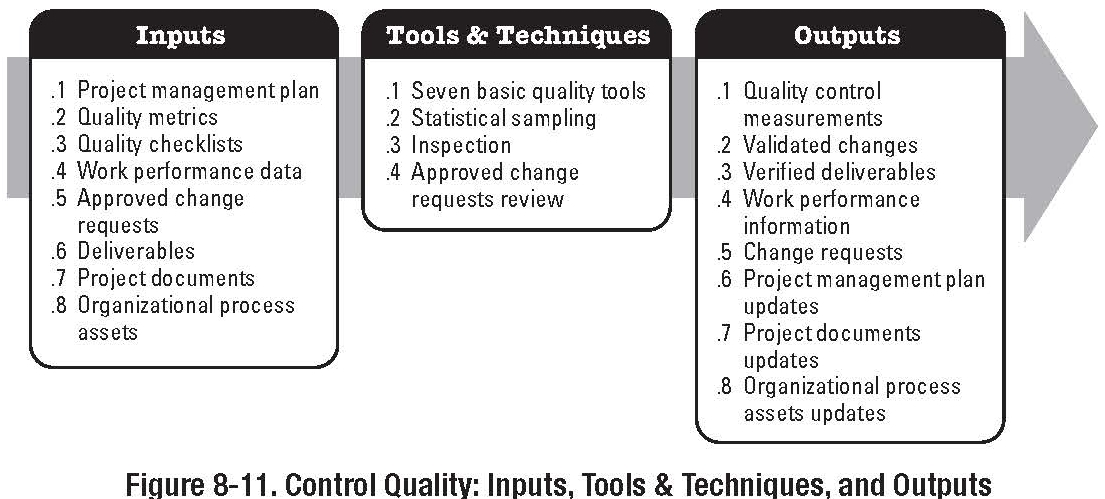
\includegraphics[width = 10cm]{images/Fig8-11.jpg}
	\label{fig:8-10}
\end{figure}
\end{frame}




\begin{frame}
\frametitle{Perform Quality Control \hfill Tools and Techniques}
\begin{itemize} 
	\item Cause and effect diagram \checkmark
	\item Control Charts 
	\item Flowcharting
	\item Histogram
	\item Pareto Chart
	\item Run Chart / Trend Analysis
	\item Scatter Diagram
	\item Statistical Sampling
	\item Inspection
	\item Defect Repair Review
\end{itemize}
\end{frame}




\begin{frame}
\frametitle{Control Charts}
\begin{figure}
	\centering
		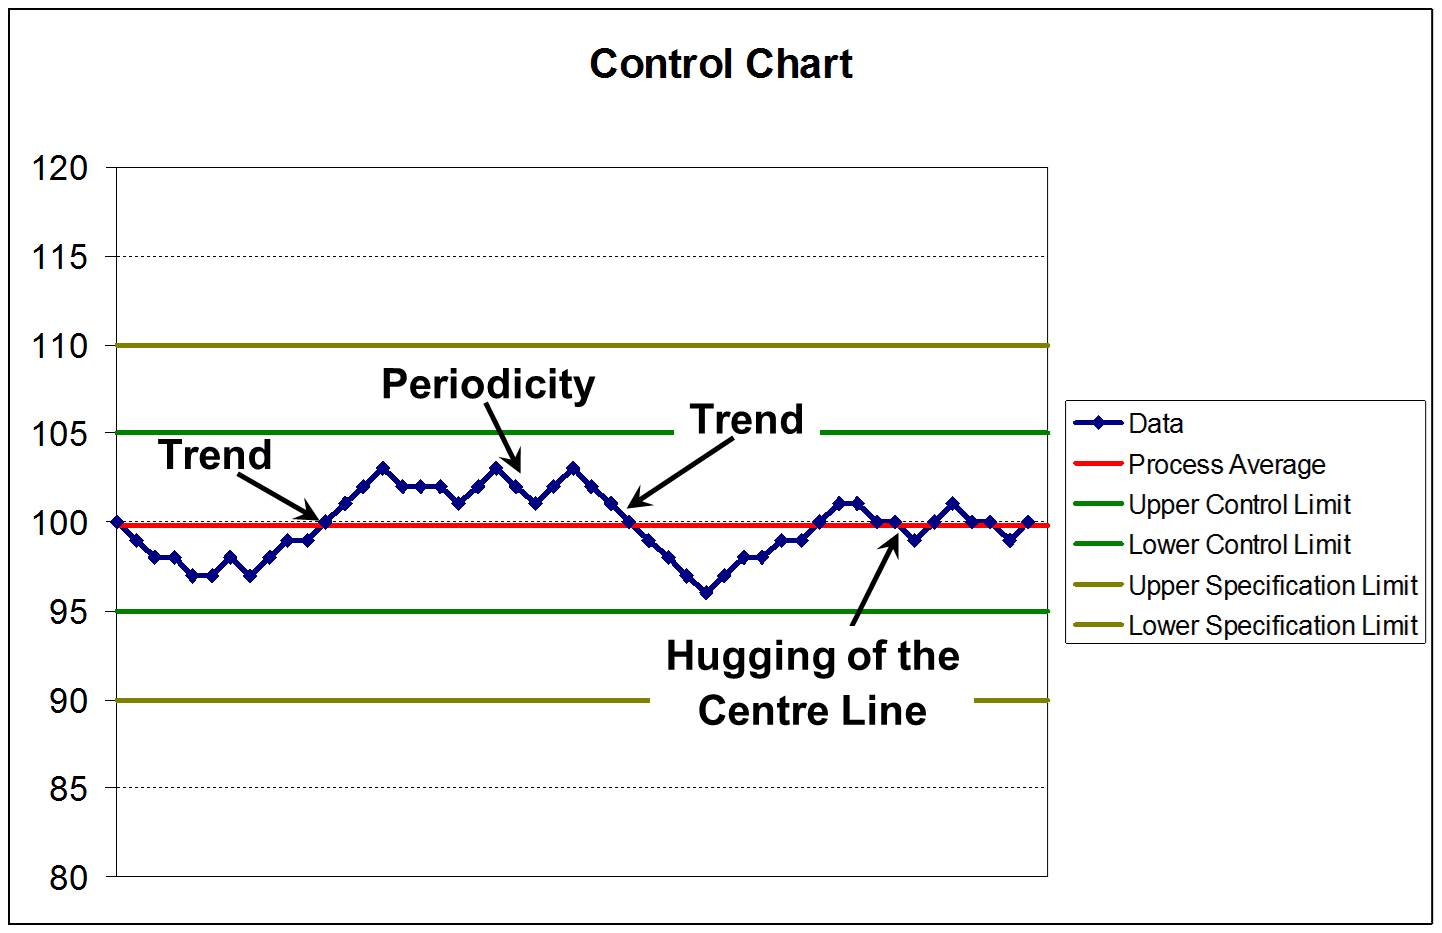
\includegraphics[width = 10cm]{images/controlchart.jpg}
	\label{fig:controlchart}
\end{figure}
\end{frame}




\begin{frame}
\frametitle{Trends}
\textbf{Trend}
\begin{itemize}
	\item If there is a continued rise or fall in a series of points, this pattern is called a trend.
	\item In general, if 7 consecutive points rise or fall, there is an abnormality.
\end{itemize}
\textbf{Periodicity}
\begin{itemize}
	\item Points that show the same pattern of change (rise or fall) over equal intervals
\end{itemize}
Hugging of the Centre Line
\begin{itemize}
	\item Points that are close to the central line, or to a control limit, are said to �hug the line�
	\item Can be indicative of a process abnormality if there is a bias.
\end{itemize}
\end{frame}



\begin{frame}
\frametitle{Pareto Diagram}
A Pareto Diagram is a specific type of histogram that is ordered by frequency of occurrence.
Organising the data in this way prioritizes the actions required to reduce non-conformance.
\begin{figure}
	\centering
		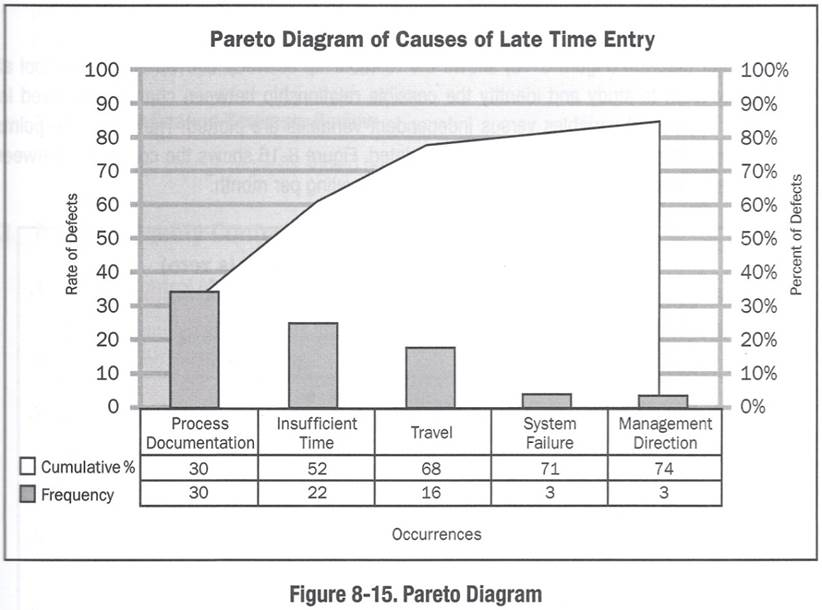
\includegraphics[width = 8cm]{images/pareto.jpg}
	\label{fig:pareto}
\end{figure}

\end{frame}




\begin{frame}
\frametitle{Pareto Analysis}
There are 3 types of Pareto Analysis:
\begin{itemize}
	\item Basic
	\item Comparative
	\item Weighted
\end{itemize}
\textbf{Basic Pareto Analysis}
\begin{itemize}
	\item Identifies the vital few contributors that account for most non-conformances
\end{itemize}
\textbf{Comparative Pareto Analysis}
\begin{itemize}
	\item Combines two or more Pareto Charts for the same process variable for comparison
\end{itemize}
\textbf{Weighted Pareto Analysis}
\begin{itemize}
	\item Applies a level of significance to other factors such as time, cost, and criticality.
\end{itemize}
\end{frame}




\begin{frame}
\frametitle{Run Chart}
Trend Analysis is performed using Run Charts
\begin{figure}
	\centering
		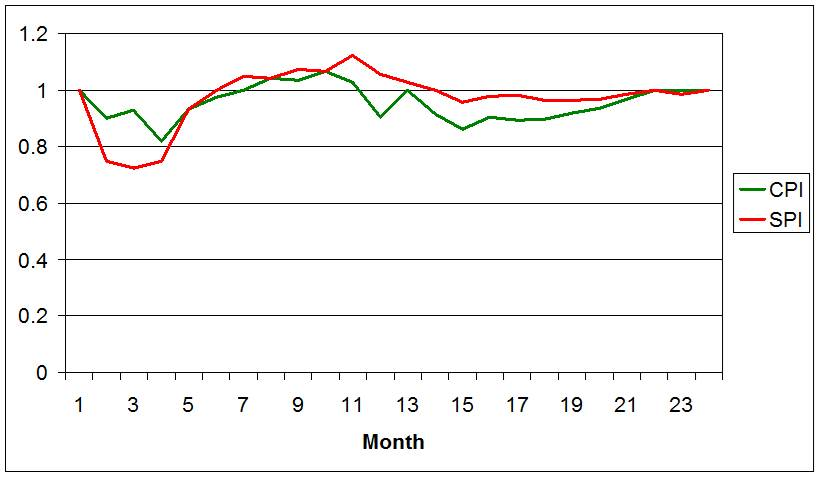
\includegraphics[width = 9cm]{images/runchart.jpg}
	\label{fig:run}
\end{figure}

\end{frame}




\begin{frame}
\frametitle{Run Chart \& Trend Analysis}
Run Chart shows:\\
\begin{itemize}
	\item History 
	\item Pattern of Variation
\end{itemize}
Run Charts show trends in processes over time.\\
Trend Analysis involves using mathematical techniques to forecast future outcomes based on historical results.\\
\end{frame}




\begin{frame}
\frametitle{Trend Analysis}
\begin{itemize}
	\item Trend Analysis is a statistical method for determining the equation that best fits the data in a scatter plot or scatter diagram.
	\item Trend Analysis quantifies the relationships of the data, determines the equation and measures the fit of the equation to the data, e.g. Curve Fitting.
	\item One of the most important aspects of trend analysis is that it can be used for forecasting
\end{itemize}
\end{frame}




\begin{frame}
\frametitle{Scatter Diagram - Student Performance}
\begin{figure}
	\centering
		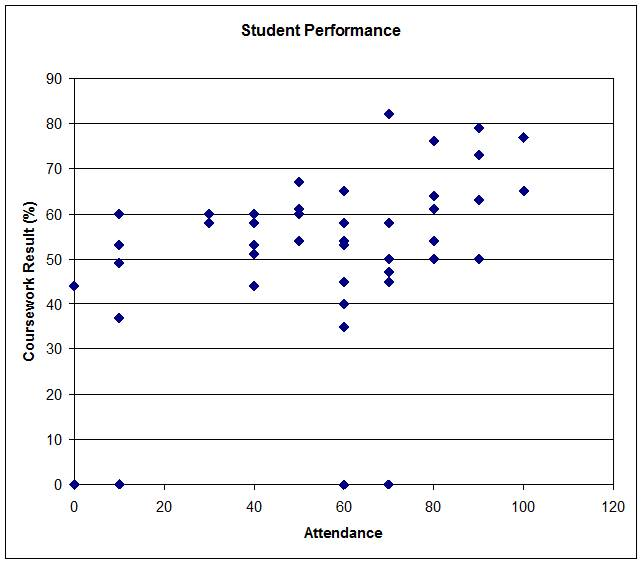
\includegraphics[width = 8cm]{images/attendscatter.jpg}
	\label{fig:studenta}
\end{figure}
\end{frame}




\begin{frame}
\frametitle{Student Performance - Trend Line}
\begin{figure}
	\centering
		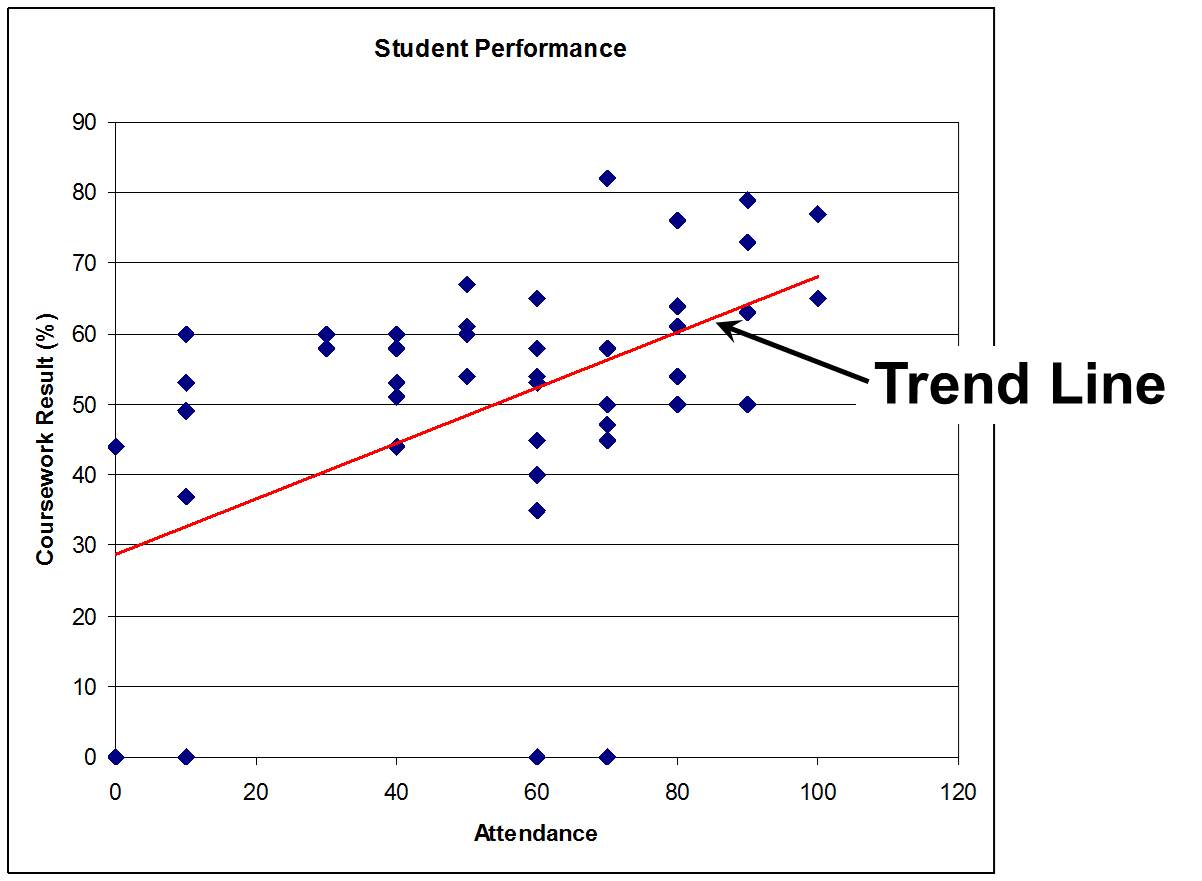
\includegraphics[width = 8cm]{images/scattertrend.jpg}
	\label{fig:studentb}
\end{figure}
\end{frame}





\begin{frame}
\frametitle{Scatter Diagram - Outliers Removed}
\begin{figure}
	\centering
		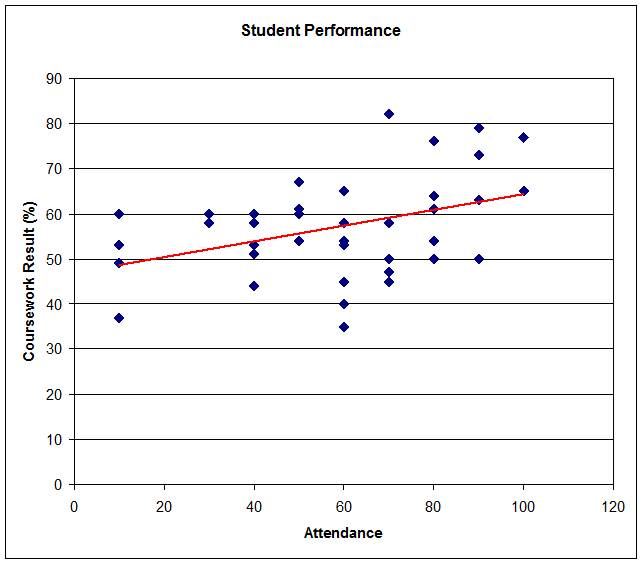
\includegraphics[width = 8cm]{images/scattertrend2.jpg}
	\label{fig:studentc}
\end{figure}
\end{frame}






\begin{frame}
\frametitle{Scatter Diagram - Polynomial}
\begin{figure}
	\centering
		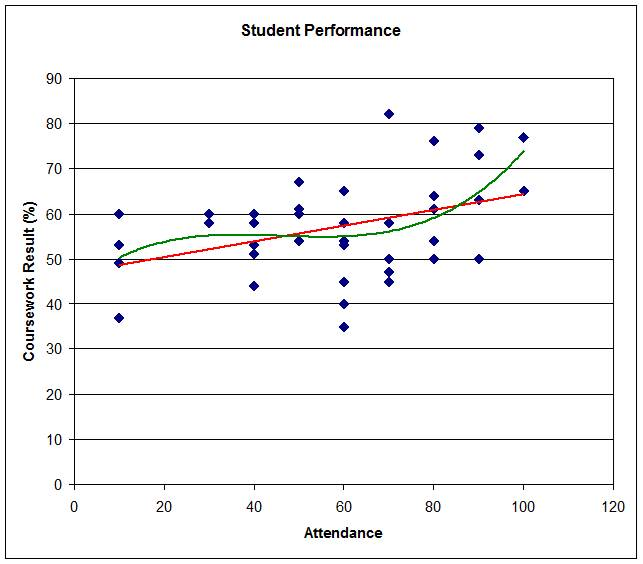
\includegraphics[width = 8cm]{images/scattertrend3.jpg}
	\label{fig:studentd}
\end{figure}
\end{frame}




\begin{frame}
\frametitle{Scatter Diagram}
Scatter diagrams organise data using two variables
\begin{itemize}
	\item An input (or independent) variable
	\item An output (or dependant) variable
\end{itemize}
The relationship between variables fall into several categories:
\begin{itemize}
	\item Positive correlation (Student Performance�.)
	\item Negative correlation
	\item Curvilinear correlation
	\item No correlation
\end{itemize}
\end{frame}




\begin{frame}
\frametitle{Statistical Sampling}
\begin{itemize}
	\item Often it is impractical or impossible to inspect all incoming or outgoing materials or products.
	\item In these instances it is more practical to randomly select a smaller number of items and test for conformance.  This is known as \textbf{acceptance sampling}
	\begin{itemize}
		\item If the sample set passes, then the lot is accepted\\
		\item If the sample set fails, the entire lot is rejected\\
	\end{itemize}
\end{itemize}
\end{frame}




\begin{frame}
\frametitle{Statistical Sampling}
\textbf{Common Sampling plans:}\\
\begin{itemize}
	\item Single Sampling - Lot is accepted or rejected based on one sampling run
	\item Double Sampling - A small sample size is tested.  If the results are not conclusive, a second sample is tested
	\item Multiple Sampling - Several small lots are sampled
\end{itemize}
\textbf{Sampling errors can occur:}
\begin{enumerate}
	\item An acceptable lot can be rejected
	\item An unacceptable lot can be accepted
\end{enumerate}
\end{frame}




\begin{frame}
\frametitle{Inspection}
\begin{itemize}
	\item Inspection is the examination of a work product to determine whether it conforms to standards.
	\item Typically involves the selection and measurement of specific characteristics.
	\item For instance timber:
		\begin{itemize}	
			\item Type
			\item Size
			\item Warp
			\item Finish
		\end{itemize}
\end{itemize}
\end{frame}




\begin{frame}
\frametitle{Defect Repair Review}
Action taken to ensure that product defects are repaired and brought into compliance with requirements or specifications
\end{frame}




\begin{frame}
\frametitle{Perform Quality Control \hfill Outputs}
\textbf{Quality Control Measurements}
\begin{itemize}
	\item Measurements that are fed back into the Quality Assurance Process
\end{itemize}
\textbf{Validated Changes}
\begin{itemize}
	\item Re-inspection after repair; results in either acceptance or rejection
\end{itemize}
\textbf{Validated Deliverables}
\begin{itemize}
	\item Validation that project deliverables conform to requirements.
\end{itemize}
\textbf{Organisational Process Assets Updates}
\begin{itemize}
	\item Completed Checklists
	\item Lessons Learned Documentation
\end{itemize}
\end{frame}




\begin{frame}
\frametitle{Perform Quality Control \hfill Outputs}
\textbf{Change Requests}
\begin{itemize}
	\item Recommended Corrective and Preventative Actions must be sent through the Integrated Change Control Process
	\item May be actions taken as a result of QC measurements
\end{itemize}
\textbf{Recommended Defect Repair}
\begin{itemize}
	\item Repair required to address a non-conformance
\end{itemize}
\textbf{Project Management Plan Updates}
\begin{itemize}
	\item Quality Management Plan
	\item Process Improvement Plan
\end{itemize}
\textbf{Project Document Updates}
\begin{itemize}
	\item Quality Standards, Procedures, Test Specs, etc.
\end{itemize}
\end{frame}



\end{document}

